\chapter{Methods}
\label{sec:methods}

The main goal of all localization systems is an estimation of the robot's pose, which describes the robot's position and orientation in space. All visual-inertial localization approaches have in common, to augment the pose estimation with the estimation of IMU characteristics and landmark positions. The methods to achieve this estimation vary over different implementations. Sections \ref{sec:rovio} and \ref{sec:okvis} will introduce the working principles and characteristics of ROVIO and OKVIS, respectively. In section \ref{sec:metrics}, the evaluation metrics are introduced, which will be used throughout this report to describe the performance of a visual-inertial localization algorithm.

\section{ROVIO}
\label{sec:rovio}

ROVIO stands for robust visual-inertial odometry and is based on an extended kalman filter (EKF), Blösch et al., \cite{bloeschrobust}. The filter state contains the robot-centric position, velocity and attitude, the accelerometer and gyroscope biases, the extrinsics between camera and IMU, and the landmarks in a robot-centric representation. Every landmark within the filter state is described with a bearing-vector and the distance between the origin of the camera frame and the landmark. The estimation is performed in two steps, leading to a tight-integration of the IMU and camera measurements. First, the filter state is propagated between two frames based on the IMU measurements. Secondly, as soon as a new image frame is available, the filter's prior belief is updated based on the camera measurement. ROVIO detects new landmarks with a FAST corner detector (Rosten et al., \cite{rosten2006machine}) and uses multilevel direct intensity patch features for landmark representation. Direct image intensity patches with a size of 8x8 pixels are extracted on different pyramid levels. If a new image is processed, the image intensity patches of the predicted features are warped and compared with the new observation to calculate a direct intensity error. This error is used for the innovation term to update the filter state. Figure \ref{pics:rovio_frontend} visualizes ROVIO during operation and gives an impression about the features that are extracted. \\

\begin{figure}
   \centering
   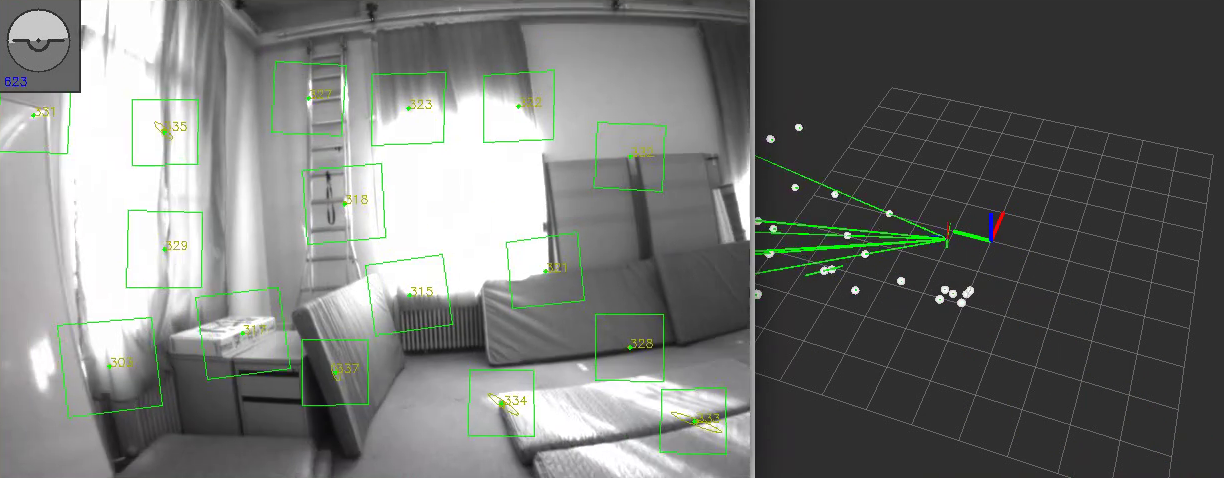
\includegraphics[width=0.9\textwidth]{images/rovio_frontend.png}
   \caption{ROVIO visualization during operation: On the left side the input image with the extracted and reprojected landmarks is shown, on the right side the fixed inertial frame (large frame), the estimated body frame (small frame) and the landmarks (white dots) with uncertainty (green lines) are visualized.}
   \label{pics:rovio_frontend}
\end{figure}

The computational complexity of an EKF scales with $O(n^3)$, where $n$ is the number of filter states, or also, in our case, the number of landmarks (Strasdat et al., \cite{strasdat2010real}). This cubic dependence is the reason, why ROVIO is working with a limited and small number of landmarks, typically between 10 and 50. To get high quality features, ROVIO has a landmark management system where features are added and removed according to a quality score based on their gradient matrix, their distance to other features and their tracking quality over the duration they have been in the filter state. 

A key assumption of the EKF approach is a gaussian distribution for the process noise and the measurement noise. The EKF performs a linearization at every update step around the filters prior belief. This step introduces linearization errors. These errors and the filtering-based property of not correcting past estimates based on new observations (see section \ref{sec:introduction}) are the main reasons why ROVIO is prone to drift.



\section{OKVIS}
\label{sec:okvis}

OKVIS stands for optimal keyframe-based visual-inertial SLAM (simultanious localization and mapping), Leutenegger et al., \cite{leutenegger2015keyframe}. OKVIS achieves the localization through tight-integration of IMU and camera measurements and performs a nonlinear optimization. The unknowns are given by the robot's position and attitude for a set of past keyframes and the newest frames on one side, and by the robot's velocity and IMU biases for the last few temporal frames on the other side. The constraints are given by the IMU measurements and the landmark observations taken by the camera. IMU error terms and reprojection error terms are combined into a single error function. OKVIS detects new features based on a multi-scale Harris corner detector (Harris et al., \cite{harris1988combined}) and describes them with a BRISK descriptor (Leutenegger et al., \cite{leutenegger2011brisk}). In order not to grow unbounded, a marginalization is performed to get rid off old keyframes and temporal frames, but keep as much useful information within the framework as possible. Figure \ref{pics:okvis_frontend} visualizes OKVIS during operation and gives an impression on the extracted features within the framework.

\begin{figure}[h]
   \centering
   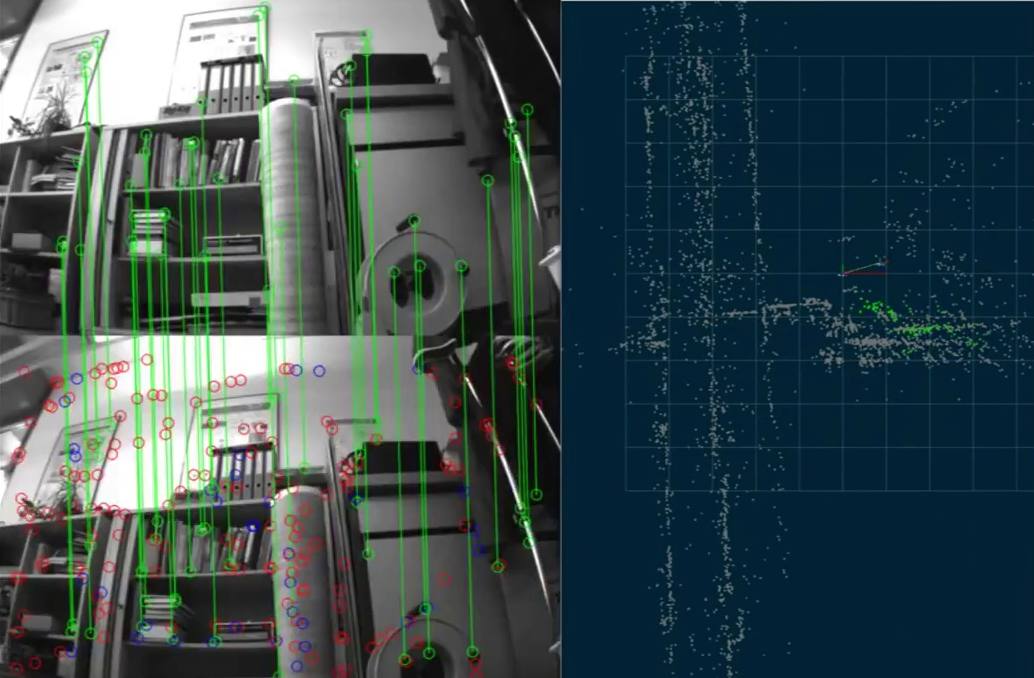
\includegraphics[width=0.6\textwidth]{images/okvis_frontend.png}
   \caption{OKVIS visualization during operation: For the latest keyframe (top) and the current frame (bottom) the extracted features are visualized with circles and the green lines denote matching pairs. Red circles stand for unmatched features, blue circles for features matched to another keyframe.}
   \label{pics:okvis_frontend}
\end{figure}

The computational complexity of bundle adjustment methods scales with $O(m^2*n)$, where $m$ is the number of keyframes and $n$ is the number of landmark observations per frame (Strasdat et al., \cite{strasdat2010real}). The number of keyframes is typically small (below 15) and the number of landmarks per frame for OKVIS is typically between 50 and 250. OKVIS is therefore executing a nonlinear optimization over a number of landmarks in the order of 1000. 

Working with more information, omitting linearization of the reprojection terms, and the keyframe-based property of allowing poses of the past to be corrected based on a new observation, make OKVIS less prone to drift. This advantage comes at the expense of a higher computational complexity.



\section{Evaluation Metrics}
\label{sec:metrics}

We propose three different metrics to evaluate the performance of a localization algorithm: global accuracy, local accuracy and computational complexity. An accurate global localization is important for long time navigation in GPS-denied environments or for indoor navigation. An accurate local localization is important for tasks like dense reconstruction or a manipulation task on a target. And the computational complexity of an algorithm is important due to the limited computational resources on an autonomous mobile robot.

To describe the global and local accuracies, the estimated pose of an algorithm is compared with a ground truth trajectory. For all evaluations in this report, the ground truth is given by an external vicon measurement system providing accurate 6D pose estimates. Working with a simplified model, we introduce an inertial coordinate frame $I$, which is world-fixed, and a body coordinate frame $B$, which is rigidly connected to the robot. 

The position of the robot with respect to $I$ is given by $_I \vec{r}_{IB} = \left[ \begin{array}{ccc} x& y& z \end{array} \right]^T$ and describes the vector from the origin of $I$ to the origin of $B$ in cartesian coordinates. 

The attitude of the robot is usually parametrized either by a rotation matrix, a triple of Euler angles, or by a unit quaternion. We will mainly use rotation matrices and, at some point, Euler angles following the Tait-Bryan convention (roll pitch yaw). Following Diebel et al. \cite{diebel2006representing}, the rotation matrix $R$, describing the attitude of the robot and hence encoding the orientation of the body frame with respect to the inertial frame, is given by 

\begin{equation}
       R = \left[ \begin{array}{ccc}
		r_{11} & r_{12}	& r_{13} \\
		r_{21} & r_{22} 	& r_{23} \\
		r_{31} & r_{32}	& r_{33} \\
		\end{array} \right]
\end{equation}

and maps a vector $_I \vec{a} $, described in world coordinates, to the same vector $_B \vec{a} $, described in body coordinates,

\begin{equation}
	_B \vec{a} = R * _I \vec{a} .
\end{equation}


The robot's pose, given by $ \left( \begin{array}{cc} _I \vec{r}_{IB}, & R \end{array} \right) $, is a function of time. We introduce the discrete time index $n$ and define the robot's pose at time index $n$ finally by 

\begin{equation}
	T(n) = \left( \begin{array}{cc} _I \vec{r}_{IB}(n), & R(n) \end{array} \right)
\end{equation}

We assume that the vicon measurement is exact and therefore supplies directly the true pose $T(n)$. To highlight the estimation of an expression we use the hat-notation. Therefore, the estimated pose is denoted by

\begin{equation}
	\hat{T}(n) = \left( \begin{array}{cc} _I \hat{\vec{r}}_{IB}(n), & \hat{R}(n) \end{array} \right) .
\end{equation}


\subsection{Global accuracy}
\label{sec:global}

To describe global accuracy, the true and estimated trajectories have to be aligned for time $n=0$ (see figure \ref{pics:absolute_relative} a) and the absolute translation error ($ATE$) and absolute orientation error ($AOE$) at time $n$ can be defined as

\begin{equation}
       ATE \left( n \right) = \left\Vert\left(\ \hat{\vec{r}} \left( n \right) - \vec{r} \left( n \right) \right) \right\Vert_2
\end{equation}
\begin{equation}
       AOE \left( n \right) = \arccos \left( \hat{R} *\vec{e_{x}} \cdot\left( R *\vec{e_{x}} \right)\right) ,
\end{equation}

where $\left\Vert \dots \right\Vert_2$ denotes the 2-norm, $\vec{e_{x}} = \left[ \begin{array}{ccc} 1& 0& 0 \end{array} \right]^T$ denotes the unit vector in $x$ direction and $\cdot$ indicates the dot-product. At some point, it will be useful to look into the 6 degrees of freedom separately and we define the absolute errors of the separated axes by

\begin{equation}
       E_{x} \left( n \right) = \left| \hat{x} \left( n \right) - x \left( n \right) \right| 
\end{equation}
\begin{equation}
       E_{y} \left( n \right) = \left| \hat{y} \left( n \right) - y \left( n \right) \right|
\end{equation}
\begin{equation}
       E_{z} \left( n \right) = \left| \hat{z} \left( n \right) - z \left( n \right) \right|
\end{equation}

\begin{equation}
	E_{\phi} \left( n \right) = \left| \hat{\phi} \left( n \right) - \phi \left( n \right)\right|
\end{equation}
\begin{equation}
	E_{\theta} \left( n \right) = \left| \hat{\theta} \left( n \right) - \theta \left( n \right)\right|
\end{equation}
\begin{equation}
	E_{\psi} \left( n \right) = \left| \hat{\psi} \left( n \right) - \psi \left( n \right)\right| ,
\end{equation}

where $\phi$, $\theta$ and $\psi$ denote the roll, pitch and yaw angles, respectively, and $\left| \dots \right|$ stands for the absolute value.


\begin{figure}
  \hspace*{1cm}
  \begin{subfigure}[b]{0.3\textwidth}
    \captionsetup{skip=6pt}
    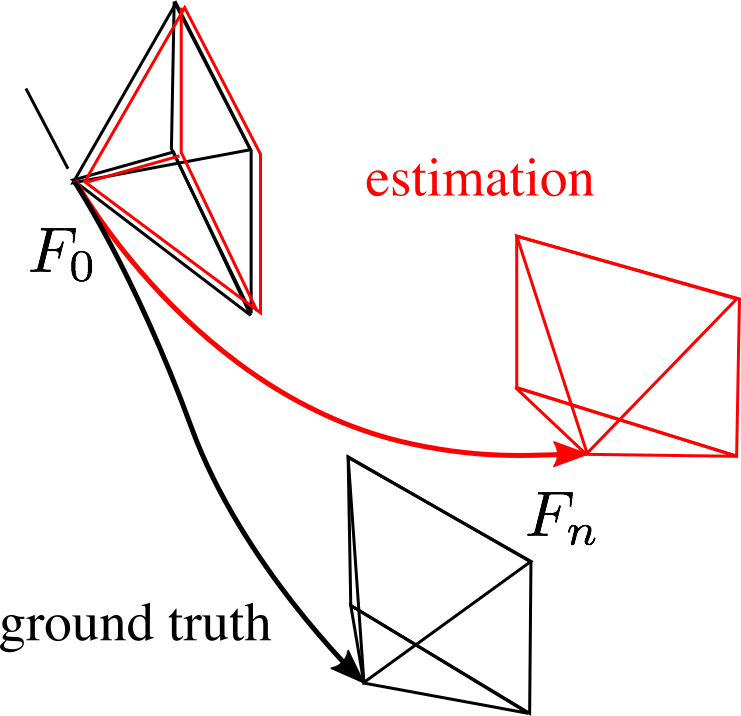
\includegraphics[width=\textwidth]{images/ape_frames_2.png}
    \caption{global accuracy}
    \label{fig:3}
  \end{subfigure}
  \hfill
  \begin{subfigure}[b]{0.28\textwidth}
    \captionsetup{skip=6pt}
    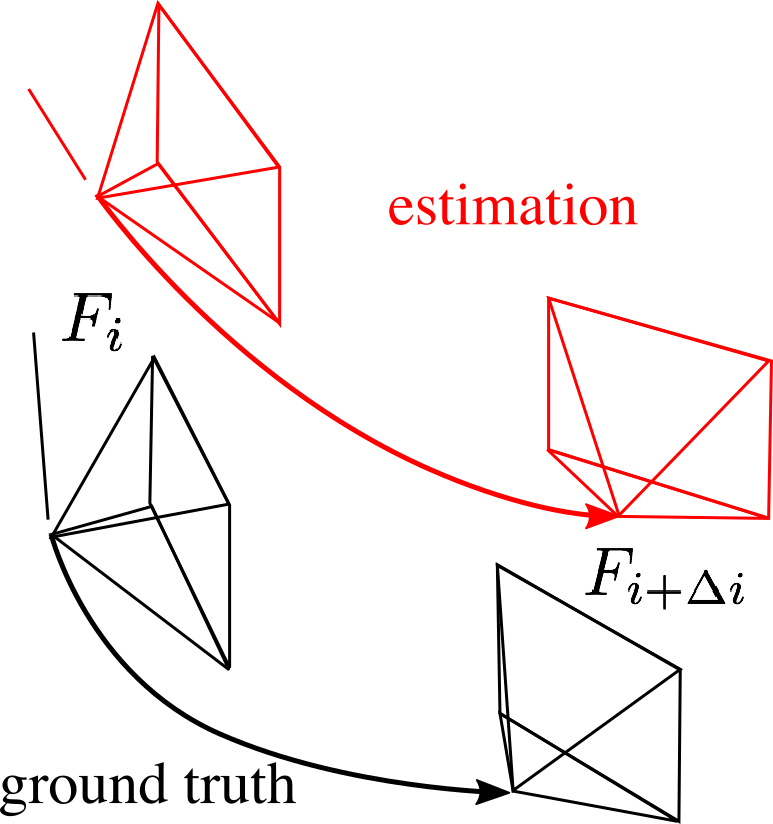
\includegraphics[width=\textwidth]{images/rpe_frames_2.png}
    \caption{local accuracy}
    \label{fig:4}
  \end{subfigure}
  \hspace*{1cm}
\caption{(a) visualizes the global accuracy: The trajectories are aligned at the first frame $F_{0}$ and the absolute difference between ground truth and estimation at time $n$ defines the global accuracy. (b) visualizes the local accuracy: The relative changes between two frames $F_i$ and $F_{i+\Delta i}$ given by the ground truth and the estimation are compared.}
\label{pics:absolute_relative}
\end{figure}





\subsection{Local accuracy}
\label{sec:local}

The local accuracy is described by relative differences between ground truth and estimation (see figure \ref{pics:absolute_relative} b). 

To describe the relative translation error, the estimated travelled distance is compared with the true travelled distance between two frames. It is a function of the frame $F_i$ at time index $i$ and the desired distance $D_{des}$. To get interesting information about the short term accuracy of the algorithm, distances between $10cm$ and $1m$ will be analysed. The relative translation error ($RTE$) is defined as

\begin{equation}
RTE \left( F_i, D_{des} \right) = \left| \hat{D} \left( F_i, F_{i+\Delta i} \right) - D \left( F_i, F_{i+\Delta i} \right)\right| ,
\end{equation}

with $ \Delta i $ such that $ D \left( F_i, F_{i+\Delta i} \right) \geq D_{des} $. The true and estimated travelled distances can be derived by summation of the incremental travelled distances between frames,

\begin{equation}
       D \left( F_i, F_{i+\Delta i} \right) = \sum_{k=i}^{i+\Delta i-1} \left\Vert\left(\ r \left( k+1 \right) - r \left( k \right) \right) \right\Vert_2
\end{equation}
\begin{equation}
       \hat{D} \left( F_i, F_{i+\Delta i} \right) = \sum_{k=i}^{i+\Delta i-1} \left\Vert\left(\ \hat{r} \left( k+1 \right) - \hat{r} \left( k \right) \right) \right\Vert_2 .
\end{equation}

To describe the local accuracy in terms of orientation, the true and estimated change in attitude are compared. The relative orientation error ($ROE$) is also a function of $F_i$ and $D_{des}$ and can be defined by

\begin{equation}
ROE\left( F_i, D_{des} \right) = \arccos \left(\left( \hat{R} \left(i\right)^T * \hat{R} \left(i+\Delta i\right) * \vec{e_{x}} \right) \cdot \left( R \left(i\right)^T * R \left(i+\Delta i\right) * \vec{e_{x}} \right)\right) .
\end{equation}

To get a statistically meaningful result on local accuracy, a number of 1000 frames $F_i$ is selected randomly out of the sequence for a desired travelled distance $D_{des}$ and the error characteristics (median, 25 and 75 percentiles, outliers) of these 1000 samples are analysed.




\subsection{Computational complexity}
\label{sec:complexity}

Beside of global and local accuracy, the third important performance measure is the computational complexity of an algorithm. Often there is a trade-off between accuracy and computational complexity.

It is common to measure computational complexity with either the CPU usage or the processing time per frame on a test system. Both metrics are dependent on the test system. The experiments for this report have been done on a 2.5GHz Intel Core 5i macbook and we will denote computational complexity with the average processing time per frame.











